\lab{Измерение удельного заряда электрона методами магнитной фокусировки и
магнетрона}

\aim{определение отношения заряда электрона к его массе методом магнитной
фокусировки и методом магнетрона.}

\labsection{А. Метод магнитной фокусировки}

\equip{электронно-лучевая трубка и блок питания к ней; соленоид; источник
постоянного тока; вольтметр;  магнитометр; ключи.}

Теоретическая часть работы изложена во введении к разделу в пункте \ref{2.1}.
%на  странице \pageref{magnetic focusing}.

\todo[inline,author=Popov,color=cyan]{Интегрировать в описание работы --->}
\paragraph{Метод магнитной фокусировки для измерения $e/m$.}
Найдём расстояние~$L$, которое проходит электрон в направлении вдоль поля за
один
оборот (шаг винтовой линии). Время одного оборота~$T_c$,
называемое \term{циклотронным периодом}, равно
$T_c= \frac{2\pi R}{v_{\perp}}$. Заменяя $R/v_{\perp}$ c помощью \eqref{3.4},
найдём
\begin{equation}
    \eqmark{3.5}
    T_c =\frac{2\pi m}{eB}.
\end{equation}

За это время электрон проходит вдоль магнитного поля расстояние
\begin{equation}
    \eqmark{3.6}
    L = v_{\parallel}T_c =\frac{2\pi v\cos\alpha}{(e/m)B}.
\end{equation}

Если углы невелики $\alpha \ll 1$, то $\cos\alpha \approx 1$ и
\begin{equation}
    \eqmark{3.7}
    L \approx \frac{2\pi v}{(e/m)B}.
\end{equation}
Таким образом, при малых углах расстояние~$L$ не зависит от~$\alpha$, так
что все электроны, вышедшие из одной точки, после одного оборота вновь соберутся
в одной точке~--- сфокусируются. Как следует из \eqref{3.7}, индукция поля~$B$,
при которой точка фокусировки отстоит от точки вылета на расстоянии~$L$, зависит
от величины~$e/m$~--- удельного заряда электрона.

Скорость движения электрона определяется разность потенциалов~$V$,
пройденную им до попадания в магнитное поле:
\begin{equation*}
  \frac{mv^2}{2}=eV,
\end{equation*}
откуда
\begin{equation}
  \eqmark{3.3}
  v=\sqrt{\frac{2eV}{m}}.
%   = 6\cdot10^5\sqrt{V}~\frac{m}{c}.
\end{equation}

Обозначим через~$B_{ф}$ индукцию магнитного поля, при которой наступает
фокусировка.
Используя \eqref{3.3} и \eqref{3.7}, выразим удельный заряд электрона~$e/m$
через~$B_{ф}$:
\begin{equation}
\eqmark{3.8}
\frac{e}{m}=\frac{8\pi^2 V}{L^2B_{ф}^2}.
\end{equation}
Эта формула положена в основу экспериментального измерения удельного заряда
электрона по \important{методу магнитной фокусировки}.
\todo[inline,color=cyan]{<---}

\todo[inline,author=Popov,color=cyan]{Интегрировать в описание работы --->}
В~так называемом {\important{методе магнетрона}} отношение~$e/m$ измеряется на
основе исследования движения электрона в скрещенных электрическом и магнитном
полях, перпендикулярных друг другу. Название метода связано с тем, что такая
конфигурация электрического и магнитного полей реализуется в магнетронах~---
генераторах электромагнитных колебаний
сверхвысоких частот.

\begin{figure}[h!]
    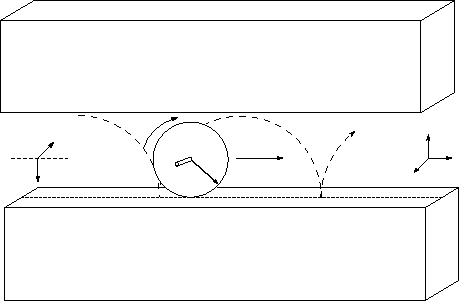
\includegraphics[width=\textwidth]{v3_3}
    \caption{Движение заряда в скрещенных полях}
    \figmark{Crossed fields}
\end{figure}
\todo[inline,author=Popov]{Рисунок странный. Что там по центру? Надо бы
нарисовать другой}

Для уяснения идеи метода магнетрона, рассмотрим вначале движение заряда в
<<плоском магнетроне>>, который можно
представить себе в виде плоского конденсатора, помещённого в магнитное поле так,
что $\vec{E}\perp\vec{B}$ (рис.~\figref{Crossed fields}). При этом отрицательная
пластина конденсатора играет роль катода, положительная соответственно анода.
Если бы магнитного поля не было, то все электроны, вылетевшие без начальной
скорости из катода такого плоского диода, попадали бы на анод. При наличии
магнитного поля траектории электронов искривляются, вследствие чего при
достаточно большом магнитном поле ни один электрон не достигнет анода. Для
заданного напряжения между катодом и анодом существует некоторое критическое
значение магнитной индукции~$B_\text{кр}$, при котором траектории касаются
поверхности анода. Если~$B<B_\text{кр}$, то все электроны достигают анода и ток
через магнетрон имеет то же значение, что и без магнитного поля. Если же
$B>B_\text{кр}$, то электроны не достигают анода и ток через лампу равен нулю.

Рассчитаем это критическое значение индукции магнитного поля. Уравнения движения
электрона в нашем случае имеет вид
\begin{equation}
    \eqmark{3.9}
    m\frac{dv_x}{dt}=ev_y B,
\end{equation}
\begin{equation}
    \eqmark{3.10}
    m\frac{dv_y}{dt}=eE-ev_x B
\end{equation}
при начальных условиях $x(0)=y(0)=0$, $v_x(0)=v_y(0)=0$.

Непосредственной подстановкой несложно убедиться в том, что решением системы
дифференциальных уравнений с заданными
начальными условиями является уравнение циклоиды (в параметрической форме):
\begin{equation}
    \eqmark{3.11}
    x = vt - R\sin\omega t,\qquad y = R(1-\cos\omega t),
\end{equation}
где $ v=E/B$, $R=v/\omega=Em/(eB^2)$.

Касание анода происходит при $2R=d$ ($d$~--- расстояние между анодом и катодом).
Этому значению соответствует
критическое поле
\begin{equation}
    B_\text{кр}=\frac{\sqrt{2V}}{d\sqrt{e/m}}.
    \eqmark{3.12}
\end{equation}
Из последней формулы находим удельный заряд:
\begin{equation}
    \eqmark{3.13}
    \frac{e}{m}=\frac{2V}{d^2B_\text{кр}^2}.
\end{equation}
\todo[inline,author=Popov]{Убрать детали в описание работы. Во введении ---
    только общие соотношения}

Эта формула позволяет вычислить~$e/m$, если при заданном значении напряжения на
аноде~$V$ найти такое значение
магнитного поля, при превышении которого ток в магнетроне отсутствует.
\todo[inline,color=cyan]{<---}

Идея опыта заключается в следующем. Электронно-лучевая трубка, вынутая из
осциллографа, помещается в длинный соленоид, создающий магнитное поле,
направленное вдоль оси трубки. Электроны вылетают из электронной пушки трубки
практически с одинаковыми продольными скоростями~$v_{\parallel}$. Небольшое
напряжение, подаваемое на отклоняющие пластины, изменяет только поперечную
составляющую скорости. Это означает, что все электроны в магнитном поле будут
двигаться по спиралям с одним и тем же шагом~$L$, и, следовательно, электроны
будут встречаться вновь, пересекая ось пучка на расстояниях~$L$,~$2L$ и т.~д.
В~этих точках сечение пучка будет наименьшим, т.~е. в них электронный пучок будет
фокусироваться. Следовательно, при изменении магнитного поля изображение пучка
на экране будет периодически стягиваться в ярко светящееся пятнышко. Если
расстояние от пушки до экрана~$l$, то пучок сфокусируется на экране при условии
$l=nL$, где $n=1,\, 2,\, 3,\, \ldots,$ или
\begin{equation*}
	l=\frac{2\pi v_{\parallel}}{\frac{e}{m} B_F}n.
\end{equation*}

Выразив в этой формуле скорость электронов через ускоряющее напряжение, получаем
выражение для удельного заряда через измеряемые физические величины:
\begin{equation}
	\frac{e}{m}=\frac{8\pi^2V}{l^2}\left(\frac{n^2}{B_F^2}\right).
	\eqmark{3.1.1}
\end{equation}

\experiment Основной частью установки является электронный осциллограф, трубка
которого вынута и установлена в длинном соленоиде, создающим магнитное поле.
Напряжение на отклоняющие пластины и питание подводятся к трубке многожильным
кабелем.Пучок электронов, вылетающих из катода с разными скоростями (энергия
электрона~$\approx 0,1$~эВ), ускоряется анодным напряжением~$\approx 1$~кВ.
После прохождения двух диафрагм из пучка выделяются электроны с практически
одинаковой продольной скоростью~$v_{\parallel}$.
\begin{figure}[h!]
	\pic{0.9\textwidth}{Chapter_3/3_1_1}
	\caption{ Схема измерений по~методу магнитной~фокусировки}
	\figmark{Magnetic focusing scheme}
\end{figure}
Небольшое переменное напряжение, подаваемое на отклоняющие пластины, изменяет
только поперечную составляющую скорости. Угол~$\alpha$ отклонения пучка от оси
трубки, таким образом, зависит от времени, и электроны прочерчивают на экране
трубки светящуюся линию. При увеличении магнитного поля линия на экране
сокращается, постепенно стягиваясь в точку, а затем снова удлиняется. Второе
прохождение через фокус происходит в том случае, когда электроны на пути от
катода к экрану описывают два витка спирали, третье~--- при трёх витках.

Анодное напряжение, определяющее продольную скорость электронов, измеряется
вольтметром.

Магнитное поле в соленоиде создаётся постоянным током
(рис.~\figref{Magnetic focusing scheme}), сила которого задается источником
питания постоянного тока и измеряется амперметром~$A$ источника. Ключ~$K$
служит для изменения направления поля в соленоиде.

Величина магнитного поля определяется с помощью магнитометра, датчик которого
расположен внутри соленоида. В~качестве магнитометра  может использоваться
милливеберметр, у которого датчиком является измерительная катушка,намотанная на
один каркас с соленоизом. Последний измеряет изменение магнитного потока,
пронизывающего измерительную катушку. Описание милливеберметра и правила работы
с ним приведены на с.~\pageref{MWB}\todo[inline,author = nozik]{Заменить ссылкой на
рисунок}.

На точность результатов может влиять внешнее магнитное поле, особенно
продольное. Оно не вызывает размытия фокуса, но изменяет величину фокусирующего
поля. Присутствие внешнего магнитного поля проще всего обнаружить с помощью
переполюсовки соленоида: при изменении направления поля показания
милливеберметра будут отличаться, но их полусумма не зависит от наличия
постоянного продольного поля.

Измерение магнитного поля обычно производится в предварительных опытах: при
отключении ключа~$K$ устанавливается связь между силой тока, протекавшего через
соленоид, и индукцией магнитного поля в соленоиде. По измеренным значениям
строится калибровочный график, который используется при обработке результатов
основных измерений для пересчёта от тока к индукции магнитного поля.

\begin{lab:task}

В~работе предлагается определить значения магнитных полей, при которых
происходит фокусировка электронного пучка, и по результатам измерений рассчитать
$e/m$.

\begin{enumerate}
\item{Ознакомьтесь с назначением ручек управления источника питания по описанию
на приборе.}
\item{Ознакомьтесь с устройством используемого в работе магнитометра}
\item{Прокалибруйте электромагнит. Для этого снимите зависимость магнитного поля
$B$ от тока~$I$ через соленоид.  В~случае использования установки с
милливеберметром,~$B$ вычисляется через поток $\Phi=BSN$, пронизывающего пробную
катушку (значение параметра~$SN$ катушки указано на установке).

Проведите указанные измерения во всем диапазоне изменения тока при двух
направлениях тока через обмотку.}
\item{При минимальном или нулевом токе через соленоид включите осциллограф  и
подайте напряжение с внешнего или внутреннего генератора на вертикальный (или
горизонтальный) вход усилителя. На экране появится светящаяся линия.}
\item{Постепенно увеличивая ток через соленоид, найдите значение тока~$I_F$, при
котором линия в первый раз стягивается в точку (сила тока~$I_F$ зависит,
конечно, от ускоряющего напряжения~$V$, а величина~$V$ меняется с изменением
яркости луча, поэтому не следует изменять яркость до конца измерений).

Продолжая увеличивать ток, снимите зависимость~$I_F$ от порядкового номера
фокуса~$n$.}
\item{ Повторите измерения $I_F=f(n)$ для другого направления магнитного поля.}
\item{ Запишите измеренное значение ускоряющего напряжения~$V$ и длину трубки
$L$, указанную на установке, и характеристики приборов.}
\item{Установите регуляторы источника питания на минимум сигнала и отключите
источник. Отключите осциллограф.}
\end{enumerate}

\tasksection{Обработка результатов}

\begin{enumerate}
\item{Постройте график $B=f(I)$.}
\item{По графику $B=f(I)$ определите усреднённые значения~$B_F$ для каждого
фокуса и постройте график зависимости $B_F=f(n)$. Используйте наклон графика для
расчёта~$e/m$ с помощью формулы~\eqref{3.1.1}.}
\item{Оцените погрешности и сравните результат с табличным.}

\end{enumerate}
\end{lab:task}

\labsection{Б. Измерение ${e/m}$ методом магнетрона}

\equip{электронная лампа с цилиндрическим анодом; источники питания лампы и
соленоида; соленоид; миллиамперметр; амперметр.}

В~настоящей работе отношение~$e/m$ для электрона определяется с помощью метода,
получившего название <<метод
магнетрона>>. Это название связано с тем, что применяемая в работе конфигурация
электрического и магнитного полей
напоминает конфигурацию полей в магнетронах~--- генераторах электромагнитных
колебаний сверхвысоких частот.

\begin{figure}[h!]
	\begin{minipage}[b]{0.49\textwidth}
		\pic{0.9\textwidth}{Chapter_3/3_1_2}
		\caption{Схема устройства двухэлектродной лампы}
		\figmark{Two-electrode lamp}
	\end{minipage}
	\hfill
	\begin{minipage}[b]{0.49\textwidth}
		\pic{0.9\textwidth}{Chapter_3/3_1_3}
		\caption{Траектории электронов, вылетающих из~катода, при~разных
значениях индукции магнитного~поля}
		\figmark{Path of electrons}
	\end{minipage}
\end{figure}

Движение электронов в этом случае происходит в кольцевом пространстве,
заключённом между катодом и анодом
двухэлектродной электронной лампы (рис.~\figref{Two-electrode lamp}). Нить
накала лампы (катод) располагается вдоль оси цилиндрического анода, так что
электрическое поле между катодом и анодом имеет радиальное направление. Лампа
помещается внутри соленоида, создающего магнитное поле, параллельное оси лампы.
Движение электронов в такой лампе рассмотрено в приложении к работе.

Рассмотрим траектории электронов, вылетевших из катода, более подробно. Пусть
потенциал анода равен~$V_A$. В~отсутствие магнитного поля (рис.~\figref{Path of
electrons}) электрон движется прямолинейно по радиусу. При слабом поле
траектории несколько искривляются, но электроны всё же попадают на анод. При
некотором критическом значении индукции магнитного поля~$B_\text{кр}$ траектории
искривляются настолько, что только касаются анода. Наконец, при~$B>B_\text{кр}$
электроны вовсе не попадают на анод и возвращаются к катоду.
Величину~$B_\text{кр}$ нетрудно найти по выведенной в приложении
формуле~\eqref{3.1.13}, заметив, что в этом случае радиальная скорость электрона
$\dot{r}$ при~$r=r_A$ (при радиусе анода) обращается в нуль:

\begin{equation}
	V_A=\frac{eB_\text{кр}^2r_A^2}{8m}.
	\eqmark{3.1.2}
\end{equation}

Преобразуя \eqref{3.1.2}, найдём
\begin{equation}
	\frac{e}{m}=\frac{8V_A}{B_\text{кр}^2r_A^2}.
	\eqmark{3.1.3}
\end{equation}

Формула~\eqref{3.1.3} позволяет вычислять~$e/m$, если при заданном~$V_A$ найдено
такое значение магнитного поля (или, наоборот, при заданном~$B$ такое значение
$V_A$), при котором электроны перестают попадать на анод.

\begin{figure}[h!]
	\pic{0.9\textwidth}{Chapter_3/3_1_4}
	\caption{Зависимость анодного тока от индукции магнитного поля в соленоиде}
	\figmark{Anode current from induction}
\end{figure}

До сих пор мы рассматривали идеальный случай, когда при $B<B_\text{кр}$ все
электроны без исключения попадают на анод, а при $B>B_\text{кр}$ все они
возвращаются на катод, не достигнув анода. Анодный ток~$I_A$ с увеличением
магнитного поля изменялся бы при этом так, как это изображено на
рис.~\figref{Anode current from induction} штриховой линией. В~реальных условиях
невозможно обеспечить полную коаксиальность анода и катода, вектор индукции
магнитного поля всегда несколько наклонён по отношению к катоду, магнитное поле
не вполне однородно и т.~д. Все эти причины приводят к сглаживанию кривой на
рис.~\figref{Anode current from induction} и она приобретает вид сплошной линии.
В~хорошо собранной установке перелом функции~$I_A=f(B)$ остаётся, однако,
достаточно резким и с успехом может быть использован для измерения~$e/m$.

\experiment Схема установки изображена на рис.~\figref{Scheme}. Двухэлектродная
лампа~$\text{Л}$ с цилиндрическим анодом специально изготовлена из немагнитных
материалов. Анод лампы состоит из трёх металлических (нержавеющая сталь)
цилиндров одинакового диаметра.
\begin{figure}[h!]
	\pic{0.9\textwidth}{Chapter_3/3_1_5}
	\caption{Схема измерительной установки}
	\figmark{Scheme}
\end{figure}
Два крайних цилиндра электрически изолированы от среднего небольшими зазорами и
используются для устранения краевых эффектов на торцах среднего цилиндра, ток с
которого используется при измерениях. В~качестве катода используется тонкая
(диаметром 50~мкм) хорошо натянутая вольфрамовая проволока, расположенная по оси
всех трёх цилиндров анодной системы. Катод лампы разогревается переменным током,
отбираемым от стабилизированного источника питания. С~другого,  регулируемого,
источника на анод лампы подаётся постоянное напряжение, измеряемое вольтметром
$V$. Ток через среднюю секцию анода измеряется с помощью миллиамперметра~$mA$.

Лампа закреплена в соленоиде. Ток, проходящий через соленоид, подаётся с
третьего источника и измеряется амперметром~$A$. Индукция магнитного поля в
соленоиде рассчитывается по току, протекающему через обмотку соленоида.
Коэффициент пропорциональности между ними указан на установке.

\begin{lab:task}

В~работе предлагается исследовать зависимость анодного тока от тока,
протекающего через соленоид, при различных
напряжениях на аноде лампы и по результатам измерений рассчитать удельный заряд
электрона.

\begin{enumerate}
\item{ Установите на аноде лампы минимальный потенциал~$V_A$, рекомендуемый в
описании конкретной установки. Снимите зависимость анодного тока~$I_A$ от
индукции магнитного поля в соленоиде (от тока~$I_{M}$ через соленоид). В~области
резкого изменения тока точки должны лежать чаще (рис.~\figref{Anode current from
induction})}.
\item{ Снимите аналогичные зависимости $I_A=f(I_M)$ для 5 -- 6 фиксированных
значений~$V_A$ в диапазоне, указанном в описании установки.}

\item{ Запишите параметры установки и характеристики приборов.}
\end{enumerate}

\tasksection{Обработка результатов}
\begin{enumerate}
\item{Используйте полученные результаты для построения семейства кривых
$I_{A}(B)$. Для каждого значения~$V_A$ определите по графику критическое
значение индукции магнитного поля~$B_\text{кр}$}.
\item Постройте  график зависимости~$B_\text{кр}^2$ от~$V_A$. По угловому
коэффициенту полученной прямой определите удельный заряд электрона~$e/m$.
Сравните результат с табличным.
\end{enumerate}
\end{lab:task}

\begin{lab:questions}
\item{ Нарисуйте и объясните схемы измерения удельного заряда электрона методом
магнитной фокусировки и методом магнетрона.}
\item{Объясните принцип действия электронно-лучевой трубки осциллографа.}
\item{ Объясните принцип работы милливеберметра.}
\item{ Почему в методе магнетрона используется анод из трёх цилиндров, а не из
одного?}
\end{lab:questions}

\begin{lab:literature}
\item{ \emph {Сивухин~Д.В.} Общий курс физики. Т. III. Электричество.~--- М.:
Физматлит, 2015, \S\S~86, 89.}
\item{ \emph {Калашников~С.Г.} Электричество.~--- М.: Физматлит, 2003,
\S\S~181--184.}
\end{lab:literature}




\labsection{Движение электрона в магнетроне}

Рассмотрим траекторию электронов, движущихся в лампе под действием
электрического и магнитного полей. Для вычислений воспользуемся цилиндрической
системой координат, т.~е. будем характеризовать положение точки расстоянием от
оси цилиндра~$r$, полярным углом~$\varphi$ и смещением вдоль оси~$z$
(рис.~\figref{Two-electrode lamp}). Рассмотрим сначала силы, действующие на
электрон со стороны электрического поля. Напряжённость электрического поля в
цилиндрическом конденсаторе имеет только радиальную компоненту~$E_r=-E$. Поэтому
сила, действующая на электрон в таком поле, направлена по радиусу, так что
\begin{equation}
	F_r^{el}=eE,\qquad F_z^{el}=F_{\varphi}^{el}=0.
	\eqmark{3.1.4}
\end{equation}

Рассмотрим теперь силы, действующие на электрон со стороны магнитного поля.
Поскольку магнитное поле в нашем случае
направлено по оси~$z$, для проекции силы на ось~$z$ имеем
\begin{equation}
	F_z^{mag}=0.
	\eqmark{3.1.5}
\end{equation}

Остальные две составляющие силы найдём с помощью формулы Лоренца. Как нетрудно
убедиться,
\begin{equation}
	F_{\varphi}^{mag}=ev_rB,\qquad F_{r}^{mag}=-ev_{\varphi}B.
	\eqmark{3.1.6}
\end{equation}

Из простых кинематических соображений ясно, что
\begin{equation}
	v_r=\dot{r}=\frac{dr}{dt},\qquad
v_{\varphi}=r\dot{\varphi}=r\frac{d\varphi}{dt}.
	\eqmark{3.1.7}
\end{equation}

Как видно из формул \eqref{3.1.4} и \eqref{3.1.5} ни магнитные, ни электрические
силы, действующие на электрон, не имеют составляющих по оси~$z$. Движение вдоль
оси~$z$ является равномерным.

Движение в плоскости ($r$,~$\varphi$) удобно описывать с помощью уравнения
моментов. Для проекции на ось~$z$ имеем
\begin{equation}
	\frac{dL_{z}}{dt}=M_z,
	\eqmark{3.1.8}
\end{equation}
где~$L_{z}$~--- момент импульса электрона относительно оси~$z$, равный, как
известно, $mr^2\dot{\varphi}$. Величина~$M_z$ равна $rF_{\varphi}$. С~помощью
\eqref{3.1.4} и \eqref{3.1.6} найдём
\begin{equation}
	M_z=erv_rB.
	\eqmark{3.1.9}
\end{equation}

Подставляя \eqref{3.1.7} и \eqref{3.1.9} в \eqref{3.1.8}, найдём
\begin{equation}
\frac{d}{dt}\left(mr^2\dot{\varphi}\right)=eBr\frac{dr}{dt}=
\frac12eB\frac{dr^2}{dt}.
	\eqmark{3.1.10}
\end{equation}

Интегрируя уравнение \eqref{3.1.10}, получаем
\begin{equation}
	r^2\dot{\varphi}+A=\frac{eBr^2}{2m},
	\eqmark{3.1.11}
\end{equation}
где~$A$~--- постоянная интегрирования, которую следует определить из начальных
условий. В~начале движения радиус~$r$ равен радиусу катода, т.~е. очень мал.
Правая часть \eqref{3.1.11} поэтому тоже очень мала. Электроны вылетают из
катода с небольшой скоростью, так что $r^{2}\dot{\varphi}$ в начальный момент
также мало. С~хорошей точностью можно поэтому полагать $A=0$. Наше уравнение
приобретает при этом простой вид:
\begin{equation}
	\dot{\varphi}=\frac{eB}{2m}.
	\eqmark{3.1.12}
\end{equation}

Рассмотрим теперь движение электрона по радиусу. Работа сил электрического поля,
совершаемая при перемещении электрона от катода до точки с потенциалом~$V$,
равна~$W=eV$. Магнитное поле никакой работы не производит. Поэтому найденная
работа должна быть равна кинетической энергии электрона (начальной скоростью
электрона мы снова пренебрегаем):
\begin{equation*}
	eV=\frac{mv^2}{2}=\frac{v_r^2+v_\varphi^2}{2m}.
\end{equation*}

С~помощью \eqref{3.1.7} и \eqref{3.1.12} найдём
\begin{equation}
	eV=\frac{m}{2}\left[\dot{r}^2+\left(\frac{reB}{2m}\right)^2\right].
	\eqmark{3.1.13}
\end{equation}

Уравнение \eqref{3.1.13} полностью определяет радиальное движение электрона.



